\documentclass[10pt,letterpaper]{article}
\usepackage[lmargin=2.2in,rmargin=0.7in,tmargin=1.0in,bmargin=1.0in]{geometry}
\usepackage{notes}
\begin{document}

\begin{center}
\Large\textbf{Day 35 –  Second Order as System, Equilibria, Linearization}\\
\normalsize (Section 5.1)
\end{center}

%%%%%%%%%%%%%%%%%%%%%%%%%%%%%%%%%%%%%%%%%%%%%%%%%%%%%%%%%%%%
\section{Rewriting Second-Order Equations}

\subsection{Motivation}
We have learned how to solve second order constant coefficient equations. However, there are many important nonlinear second order differential equations which cannot be solved. Here are a few important nonlinear models:
\begin{itemize}
    \item 
\end{itemize}
Although we cannot solve them, we can still plot their phase portraits! First, we must learn how to rewrite second order equations in matrix form. 


\subsection{Matrix Form}
Consider the equation
$$
    x''+7x'+12x=0
$$
The characteristic eqution is ... the eigenvalues are... 
Now what if we introduce a new variable $y=x'$ what happens is...
wow its a matrix equation $x'=Ax$. 




\begin{example}[1]{
Rewrite the equation as a first order system
\[
(nonlinear example) 
\]
}

rewrite 
\end{example}

The matrix and the original second-order equation
have the same characteristic polynomial. This explains
why the two methods produce the same eigenvalues
and solution.

\subsection{General Theory}
Suppose you have the general system
$$ax''+bx'+cx=f(x)$$
THis is how you can convert it to a system.

Introduce a new variable
\[
y(t)=x'(t).
\]
Then $y'=x''$, so
\[
x''+bx'+cx=0
\quad\Longleftrightarrow\quad
\begin{dcases}
x'=y,\\
y'=-cx-by.
\end{dcases}
\]
In matrix form,
\[
\boxed{
\mathbf{x}'=
\begin{pmatrix}
0&1\\
-c&-b
\end{pmatrix}\mathbf{x},
\qquad
\mathbf{x}=
\begin{pmatrix}x\\y\end{pmatrix}.
}
\]
The first component is the original unknown $x(t)$;
the second is its derivative.

Initial conditions translate directly:
\[
x(0)=x_0,\qquad x'(0)=v_0
\quad\Longleftrightarrow\quad
\mathbf{x}(0)=
\begin{pmatrix}x_0\\v_0\end{pmatrix}.
\]
\subsection{What now?}
The system we wrote is nonlinear! How do we plot its phase?

%%%%%%%%%%%%%%%%%%%%%%%%%%%%%%%%%%%%%%%%%%%%%%%%%%%%%%%%%%%%%
\section{Nonlinear Systems}

\subsection{The Equilibria}

A two-dimensional \textbf{autonomous system} has the form
\[
\begin{dcases}
x'=F_1(x,y),\\
y'=F_2(x,y).
\end{dcases}
\]
In vector notation,
\[
\boxed{
\mathbf{x}'=\mathbf{F}(\mathbf{x}),
\qquad
\mathbf{F}(x,y)=
\begin{pmatrix}
F_1(x,y)\\
F_2(x,y)
\end{pmatrix}.
}
\]
The word \textit{autonomous} means that the right-hand
side does not explicitly depend on time $t$. 

An \textbf{equilibrium} is a point $\mathbf{x}^*$ where
\[
\mathbf{F}(\mathbf{x}^*)=\mathbf{0}.
\]

%-------------------------------------------------------------
\subsection{Linear versus Nonliear Systems}

The systems we have studied so far have the form
\[
\mathbf{x}'=A\mathbf{x}
=
\begin{pmatrix}
ax+by\\
cx+dy
\end{pmatrix}.
\]
These are homogeneous linear systems.

The origin is always an equilibrium. If $A$ is
invertible, it is the only equilibrium.

We can also include a constant forcing vector:
\[
\mathbf{x}'=A\mathbf{x}+\mathbf{b}.
\]
This is a nonhomogeneous linear system. Strictly speaking,
the map $A\mathbf{x}+\mathbf{b}$ is \textit{affine}
when $\mathbf{b}\ne\mathbf{0}$.

Its equilibria satisfy
\[
A\mathbf{x}^*+\mathbf{b}=\mathbf{0}.
\]
If $A$ is invertible, the unique equilibrium is
\[
\boxed{\mathbf{x}^*=-A^{-1}\mathbf{b}.}
\]
We will see that its phase portrait is a translated
version of the portrait for $\mathbf{u}'=A\mathbf{u}$.

A system is \textbf{nonlinear} if its right-hand side
contains nonlinear dependence on the unknowns, such as
$x^2$, $xy$, or $\sin x$.

For example,
\[
\mathbf{x}'=
\begin{pmatrix}
y-x^2\\
x(1-y)
\end{pmatrix}
\]
is nonlinear.

Many nonlinear systems are difficult to solve explicitly.
However, we can still study their equilibria and sketch
the behavior of nearby solutions.


%-------------------------------------------------------------
\subsection{Finding Equilibria}
Key differenece is that nonlinears can be multiple equilibria.

To find equilibria, solve both equations simultaneously:
\[
F_1(x,y)=0,\qquad F_2(x,y)=0.
\]
Unlike an invertible homogeneous linear system,
a nonlinear system can have several isolated equilibria.

\begin{example}[2]{
Find all equilibria:
\[
\mathbf{x}'=
\begin{pmatrix}
y-x^2\\
x(1-y)
\end{pmatrix}.
\]
}

\paragraph{Step 1. Set both components equal to zero.}
We need
\[
y-x^2=0,
\qquad
x(1-y)=0.
\]
The second equation gives two cases:
\[
x=0\qquad\text{or}\qquad y=1.
\]

\paragraph{Step 2. Check each case in the first equation.}
If $x=0$, then
\[
y-x^2=y=0,
\]
giving $(0,0)$.

If $y=1$, then
\[
1-x^2=0
\implies x=\pm1,
\]
giving $(1,1)$ and $(-1,1)$.

Therefore, the equilibria are
\[
\boxed{(0,0),\qquad (1,1),\qquad (-1,1).}
\]
\end{example}


%%%%%%%%%%%%%%%%%%%%%%%%%%%%%%%%%%%%%%%%%%%%%%%%%%%%%%%%%%%%%%%%
\section{Linearization}

\subsection{Phase Portrait for Nonlinear Systems}
Suppose a nonlinear system has two equilibria x0 and x1. Each equilibria is associated with its \textit{own local matrix} A0 and A1. To sketch the phase diagram for the nonlinear system we must do what we did in chapter 4. classify the two equilibria based on the eigenvalues of A0 and A1. Then we sketch local, orbits near x0 and x1 based on their classification. 

\begin{figure}[H]
    \centering
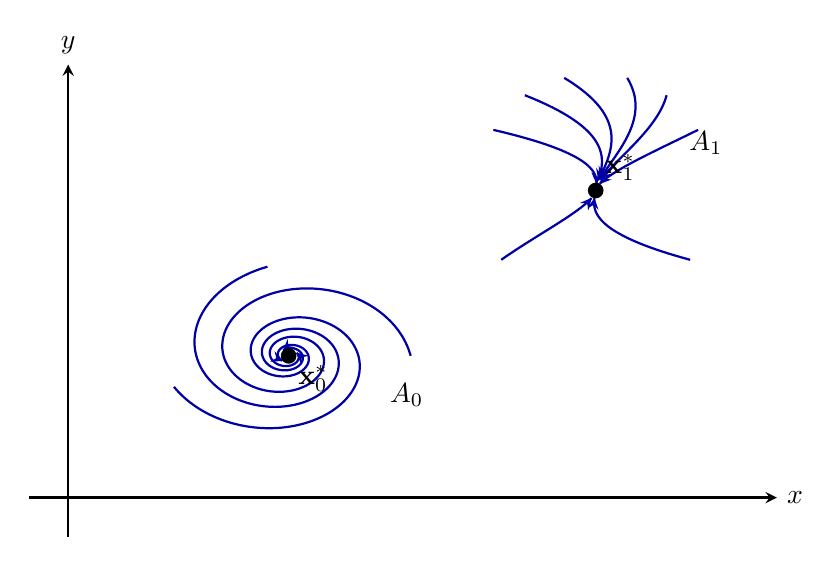
\begin{tikzpicture}[
    >=stealth,
    scale=1,
    trajectory/.style={thick, blue!65!black},
    equilibrium/.style={circle, fill=black, inner sep=2pt}
]

% Coordinate axes
\draw[->, thick] (-0.5,0) -- (9,0) node[right] {$x$};
\draw[->, thick] (0,-0.5) -- (0,5.5) node[above] {$y$};

% Equilibria
\coordinate (P0) at (2.8,1.8);
\coordinate (P1) at (6.7,3.9);

% Stable spiral around P0
\begin{scope}[shift={(P0)}]
    \foreach \phase in {0,100,200} {
        \draw[trajectory, ->, domain=0:750,
              samples=180, smooth, variable=\t]
            plot ({
                (1.55*exp(-0.0035*\t))*
                cos(\t+\phase)
            },{
                (1.15*exp(-0.0035*\t))*
                sin(\t+\phase)
            });
    }
\end{scope}

% Stable node around P1
% Curved trajectories approaching the equilibrium
\begin{scope}[shift={(P1)}]
    \foreach \a/\b in {
        -1.3/0.7,
        -0.9/1.1,
        -0.4/1.3,
         0.4/1.3,
         0.9/1.1,
         1.3/0.7,
        -1.2/-0.8,
         1.2/-0.8
    } {
        \draw[trajectory, ->,
              domain=0:2.8, samples=65,
              smooth, variable=\t]
            plot ({
                \a*exp(-1.5*\t)
                + \b*\t*exp(-1.5*\t)
            },{
                1.1*\b*exp(-0.8*\t)
            });
    }
\end{scope}

% Equilibrium markers
\node[equilibrium] at (P0) {};
\node[equilibrium] at (P1) {};

% Labels
\node[below right] at (P0) {$\mathbf{x}_0^*$};
\node[above right] at (P1) {$\mathbf{x}_1^*$};

\node at (4.3,1.3) {$A_0$};
\node at (8.1,4.5) {$A_1$};
\end{tikzpicture}
\end{figure}



%------------------------------------------------------
\subsection{The Jacobian Matrix}

But what exactly are these matrices A0 and A1?
For a vector-valued function
\[
\mathbf{F}(x,y)=
\begin{pmatrix}
F_1(x,y)\\
F_2(x,y)
\end{pmatrix},
\]
the \textbf{Jacobian matrix} contains its four first-order
partial derivatives:
\[
\boxed{
J(x,y)=
\begin{pmatrix}
\dfrac{\partial F_1}{\partial x}
&
\dfrac{\partial F_1}{\partial y}\\[6pt]
\dfrac{\partial F_2}{\partial x}
&
\dfrac{\partial F_2}{\partial y}
\end{pmatrix}.
}
\]
Each row comes from one component of $\mathbf{F}$.

\begin{example}[3]{
Find the Jacobian of
\[
\mathbf{F}(x,y)=
\begin{pmatrix}
y-x^2\\
x(1-y)
\end{pmatrix}.
\]
}
The partial derivatives are
\[
\frac{\partial F_1}{\partial x}=-2x,
\qquad
\frac{\partial F_1}{\partial y}=1,
\]
and
\[
\frac{\partial F_2}{\partial x}=1-y,
\qquad
\frac{\partial F_2}{\partial y}=-x.
\]
Therefore,
\[
\boxed{
J(x,y)=
\begin{pmatrix}
-2x&1\\
1-y&-x
\end{pmatrix}.
}
\]
\end{example}

%--------------------------------------------------------
\subsection{Local Behavior Near an Equilibrium}

Suppose x0 is an equilibrium for a nonlinear system x'=F(x). 
To find the local behavior centered at x0, calculate the Jacobian of F(x).
Then plug x0 into F(x). The matrix A0 = F(x) is what controls the local behavior of the solution near x0. 

To sketch a phase for a nonliear system:
a) find all equis
b) find jacobian
c) for each equi, plug x* into J and classify local matrix 
d) for eahc equi, sketch local orbits like we've done in chap 4 

%--------------------------------------------------------

\subsection{How does the Jacobian Work (just going to rush this in actual lecture)}

To understand the Jacobian, it helps to think of the 1D version.
Near a point $x_0$, we can approximate a differentiable
function by its tangent line:
\[
\boxed{
f(x)\approx f(x_0)+f'(x_0)(x-x_0).
}
\]
This is called \textbf{linearization}.

For example, consider
\[
x'=f(x)=x^2-4.
\]
The point $x^*=2$ is an equilibrium because $f(2)=0$.
Since $f'(2)=4$, near this equilibrium,
\[
x'\approx4(x-2).
\]
Setting $u=x-2$ gives the linearized equation
\[
u'=4u.
\]
Its solutions move away from $u=0$, suggesting that
the original equilibrium $x^*=2$ is unstable.
The goal is to understand a nonlinear equation near
an equilibrium by studying a simpler linear equation.

So the Jacobian is the derivative term in the 2d version of linearization.
The two-dimensional linear approximation is
\[
\mathbf{F}(\mathbf{x})
\approx
\mathbf{F}(\mathbf{x}^*)
+J(\mathbf{x}^*)(\mathbf{x}-\mathbf{x}^*).
\]
At an equilibrium, $\mathbf{F}(\mathbf{x}^*)=\mathbf{0}$.
Thus,
\[
\mathbf{x}'\approx
J(\mathbf{x}^*)(\mathbf{x}-\mathbf{x}^*).
\]

Introduce coordinates measured from the equilibrium:
\[
\mathbf{u}=\mathbf{x}-\mathbf{x}^*.
\]
Because $\mathbf{x}^*$ is constant,
$\mathbf{u}'=\mathbf{x}'$. The resulting
\textbf{linearized system} is
\[
\boxed{
\mathbf{u}'=J(\mathbf{x}^*)\mathbf{u}.
}
\]
The equilibrium $\mathbf{x}^*$ becomes the origin
in the $\mathbf{u}$-coordinates.

We analyze this linear system using eigenvalues
and eigenvectors, then place the resulting local
picture at $\mathbf{x}^*$.

%%%%%%%%%%%%%%%%%%%%%%%%%%%%%%%%%%%%%%%%%%%%%%%%%%%%%%%%%%%%%%%%%%%%%%%%
\section{Sketching Local Orbits}

\subsection{Translating the Equilibrium}

For the system
\[
\mathbf{x}'=A\mathbf{x}+\mathbf{b},
\]
suppose $\mathbf{x}^*$ is an equilibrium. Set
$\mathbf{u}=\mathbf{x}-\mathbf{x}^*$. Then
\begin{align*}
\mathbf{u}'
&=A(\mathbf{u}+\mathbf{x}^*)+\mathbf{b}\\
&=A\mathbf{u}
+\underbrace{A\mathbf{x}^*+\mathbf{b}}_{\mathbf{0}}\\
&=A\mathbf{u}.
\end{align*}
Here, the transformation is \textbf{exact}.
There are no nonlinear terms to discard.

The phase portrait is the portrait for
$\mathbf{u}'=A\mathbf{u}$ translated so its equilibrium
lies at $\mathbf{x}^*$.

%-------------------------------------------------------------
\subsection{A Shifted Saddle}

\begin{example}[4]{
Find the equilibrium and sketch the phase portrait:
\[
\mathbf{x}'=
\begin{pmatrix}
-3&1\\
-4&2
\end{pmatrix}\mathbf{x}
+
\begin{pmatrix}2\\2\end{pmatrix}.
\]
}

\paragraph{Step 1. Find the equilibrium.}
Set the right-hand side equal to zero:
\[
\begin{dcases}
-3x+y+2=0,\\
-4x+2y+2=0.
\end{dcases}
\]
The first equation gives $y=3x-2$. Substituting
into the second,
\[
-4x+2(3x-2)+2=0
\implies x=1,\qquad y=1.
\]
Thus,
\[
\boxed{
\mathbf{x}^*=\begin{pmatrix}1\\1\end{pmatrix}.
}
\]

\paragraph{Step 2. Shift the equilibrium to the origin.}
Let
\[
\mathbf{u}=
\mathbf{x}-\begin{pmatrix}1\\1\end{pmatrix}.
\]
Then
\[
\mathbf{u}'=
\begin{pmatrix}
-3&1\\
-4&2
\end{pmatrix}\mathbf{u}.
\]

\paragraph{Step 3. Find the eigenvalues and eigenvectors.}
The characteristic equation is
\[
\begin{vmatrix}
\lambda+3&-1\\
4&\lambda-2
\end{vmatrix}
=\lambda^2+\lambda-2
=(\lambda+2)(\lambda-1)=0.
\]
The eigenpairs are
\[
\lambda_1=-2,\qquad
\mathbf{v}_1=\begin{pmatrix}1\\1\end{pmatrix},
\]
and
\[
\lambda_2=1,\qquad
\mathbf{v}_2=\begin{pmatrix}1\\4\end{pmatrix}.
\]
Since the eigenvalues have opposite signs,
\[
\boxed{(1,1)\text{ is a saddle}.}
\]

\paragraph{Step 4. Sketch the translated phase portrait.}
Draw the eigenvector lines through $(1,1)$:
\begin{itemize}
    \item Stable direction:
    $y-1=x-1$, with arrows toward $(1,1)$.
    \item Unstable direction:
    $y-1=4(x-1)$, with arrows away from $(1,1)$.
\end{itemize}
The general solution is
\[
\mathbf{x}(t)=
\begin{pmatrix}1\\1\end{pmatrix}
+c_1e^{-2t}\begin{pmatrix}1\\1\end{pmatrix}
+c_2e^t\begin{pmatrix}1\\4\end{pmatrix}.
\]

\begin{center}
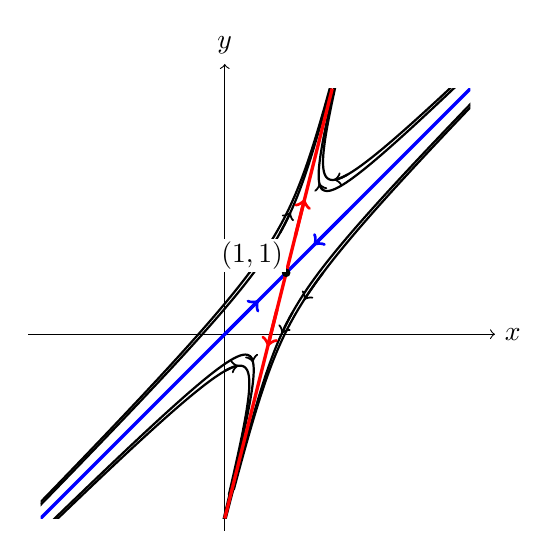
\begin{tikzpicture}[scale=0.78]
    % Axes
    \draw[->] (-3.2,0)--(4.4,0) node[right] {$x$};
    \draw[->] (0,-3.2)--(0,4.4) node[above] {$y$};

    \begin{scope}
    \clip (-3,-3) rectangle (4,4);

    % Exact solution curves
    \foreach \c/\d in {
        0.35/0.25,0.35/-0.25,
        -0.35/0.25,-0.35/-0.25,
        0.8/0.2,0.8/-0.2,
        -0.8/0.2,-0.8/-0.2
    }{
        \draw[thick,domain=-1.7:1.5,samples=200]
            plot
            ({1+\c*exp(-2*\x)+\d*exp(\x)},
             {1+\c*exp(-2*\x)+4*\d*exp(\x)});

        \draw[thick,->,domain=0:0.2,samples=20]
            plot
            ({1+\c*exp(-2*\x)+\d*exp(\x)},
             {1+\c*exp(-2*\x)+4*\d*exp(\x)});
    }

    % Stable and unstable lines
    \draw[blue,very thick] (-3,-3)--(4,4);
    \draw[red,very thick] (0,-3)--(1.75,4);

    % Stable arrows
    \draw[blue,very thick,->] (2,2)--(1.45,1.45);
    \draw[blue,very thick,->] (0,0)--(0.55,0.55);

    % Unstable arrows
    \draw[red,very thick,->] (1.15,1.6)--(1.3,2.2);
    \draw[red,very thick,->] (0.85,0.4)--(0.7,-0.2);
    \end{scope}

    \fill (1,1) circle (2pt);
    \node[above left,fill=white,inner sep=1pt]
        at (1,1) {$(1,1)$};
\end{tikzpicture}

\small
Blue: stable direction.
Red: unstable direction.
\end{center}
\end{example}



\subsection{Nonlinear Example}

For a nonlinear system, we repeat the linearization
procedure at each equilibrium. Different equilibria
can have different classifications.

\begin{example}[5]{
Find and classify the equilibria of
\[
\begin{dcases}
x'=x-y,\\
y'=2y(y-1).
\end{dcases}
\]
Find the eigendirections of each linearized system
and sketch the local behavior.
}

\paragraph{Step 1. Find the equilibria.}
Solve
\[
x-y=0,\qquad 2y(y-1)=0.
\]
The second equation gives $y=0$ or $y=1$.
Since $x=y$, the equilibria are
\[
\boxed{(0,0)\qquad\text{and}\qquad(1,1).}
\]

\paragraph{Step 2. Compute the Jacobian.}
With
\[
F_1(x,y)=x-y,\qquad F_2(x,y)=2y^2-2y,
\]
we obtain
\[
J(x,y)=
\begin{pmatrix}
1&-1\\
0&4y-2
\end{pmatrix}.
\]

\paragraph{Step 3. Classify the equilibrium at $(0,0)$.}
At the origin,
\[
A_1=J(0,0)=
\begin{pmatrix}
1&-1\\
0&-2
\end{pmatrix}.
\]
Since this matrix is triangular, its eigenvalues
are its diagonal entries:
\[
\lambda_1=1,\qquad \lambda_2=-2.
\]
The corresponding eigenvectors are
\[
\lambda_1=1:
\quad
\mathbf{v}_1=\begin{pmatrix}1\\0\end{pmatrix},
\qquad
\lambda_2=-2:
\quad
\mathbf{v}_2=\begin{pmatrix}1\\3\end{pmatrix}.
\]
Therefore,
\[
\boxed{(0,0)\text{ is a saddle}.}
\]
The linearized system has:
\begin{itemize}
    \item an unstable direction along $(1,0)$;
    \item a stable direction along $(1,3)$.
\end{itemize}

\paragraph{Step 4. Classify the equilibrium at $(1,1)$.}
At the second equilibrium,
\[
A_2=J(1,1)=
\begin{pmatrix}
1&-1\\
0&2
\end{pmatrix}.
\]
Its eigenvalues and eigenvectors are
\[
\lambda_1=1:
\quad
\mathbf{v}_1=\begin{pmatrix}1\\0\end{pmatrix},
\qquad
\lambda_2=2:
\quad
\mathbf{v}_2=\begin{pmatrix}-1\\1\end{pmatrix}.
\]
Both eigenvalues are positive, so
\[
\boxed{(1,1)\text{ is an unstable node}.}
\]
Both eigendirections point outward. Generic trajectories
of the linearized system are tangent to the slower
direction $(1,0)$ near the equilibrium.

\paragraph{Step 5. Sketch the local directions.}
Place each local picture at its equilibrium.
Use short segments to show the eigendirections
and arrows to indicate motion.

\begin{center}
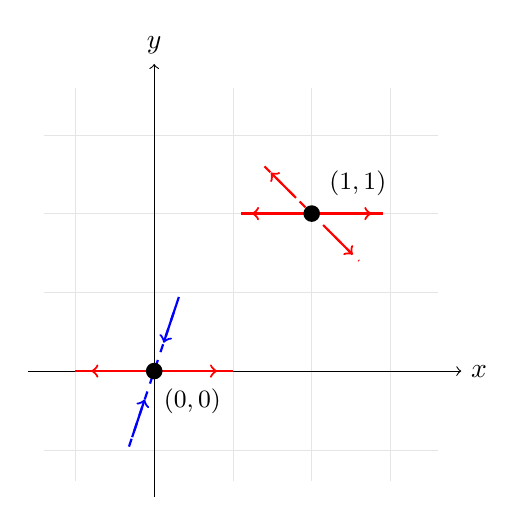
\begin{tikzpicture}[scale=2.0]
    % Grid and axes
    \draw[step=0.5,very thin,gray!20]
        (-0.7,-0.7) grid (1.8,1.8);
    \draw[->] (-0.8,0)--(1.95,0) node[right] {$x$};
    \draw[->] (0,-0.8)--(0,1.95) node[above] {$y$};

    % Saddle at (0,0): unstable direction
    \draw[red,thick] (-0.5,0)--(0.5,0);
    \draw[red,thick,->] (0.15,0)--(0.4,0);
    \draw[red,thick,->] (-0.15,0)--(-0.4,0);

    % Saddle at (0,0): stable tangent direction
    \draw[blue,dashed,thick] (-0.16,-0.48)--(0.16,0.48);
    \draw[blue,thick,->] (0.14,0.42)--(0.06,0.18);
    \draw[blue,thick,->] (-0.14,-0.42)--(-0.06,-0.18);

    % Node at (1,1): horizontal direction
    \draw[red,thick] (0.55,1)--(1.45,1);
    \draw[red,thick,->] (1.12,1)--(1.38,1);
    \draw[red,thick,->] (0.88,1)--(0.62,1);

    % Node at (1,1): other tangent direction
    \draw[red,dashed,thick] (0.7,1.3)--(1.3,0.7);
    \draw[red,thick,->] (0.9,1.1)--(0.74,1.26);
    \draw[red,thick,->] (1.1,0.9)--(1.26,0.74);

    % Equilibria
    \fill (0,0) circle (1.5pt);
    \fill (1,1) circle (1.5pt);
    \node[below right] at (0,-0.05) {\small $(0,0)$};
    \node[above right] at (1.05,1.05) {\small $(1,1)$};
\end{tikzpicture}

\small
Local eigendirections at the two equilibria.
Blue arrows point inward; red arrows point outward.
Dashed lines show tangent directions.
\end{center}
\end{example}


%%%%%%%%%%%%%%%%%%%%%%%%%%%%%%%%%%%%%%%%%%%%%%%%%%%%
\section{Extending Local Orbits}
%%%%%%%%%%%%%%%%%%%%%%%%%%%%%%%%%%%%%%%%%%%%%%%%%%%%

%-------------------------------------------------------------
\subsection{Local Directions Are Not Always Straight Trajectories}

For a linear system, eigenvectors give exact
straight-line trajectories. For a nonlinear system,
they generally give \textbf{tangent directions}
near an equilibrium. The actual trajectories may curve.

In Example 5, the horizontal lines $y=0$ and $y=1$
are invariant because $y'=0$ on both lines.
The other eigendirections are local approximations,
not exact straight-line trajectories.

%-------------------------------------------------------------
\subsection{Beyond the Equilibria}

Linearization describes behavior near each equilibrium.
To extend the sketch farther away, use information
from the original system:
\[
x'=x-y,\qquad y'=2y(y-1).
\]
For Example 5,
\begin{itemize}
    \item $x>y$ gives motion to the right;
    $x<y$ gives motion to the left.
    \item $y<0$ or $y>1$ gives upward motion.
    \item $0<y<1$ gives downward motion.
\end{itemize}

These directions help guide a larger phase portrait.
Distinct trajectories cannot cross because this smooth
system has unique solutions.

However, local sketches alone do not determine how
trajectories connect across the phase plane.
Use the original vector field or numerical solutions
when more detail is needed.

%%%%%%%%%%%%%%%%%%%%%%%%%%%%%%%%%%%%%%%%%%%%%%%%%%%%%%%%%%%%%%%%%%%%%%%%

Sketch the phase portrait of the nonlinear system
\[
\begin{cases}
x' = x - y,\\[3pt]
y' = 2y(-1+y).
\end{cases}
\]

\subsection*{Step 1: Find all equilibria.}
To find the equilibria, solve
\[
\mathbf{F}(x,y)=\mathbf{0}.
\]
That is,
\[
x-y=0,
\qquad
2y(-1+y)=0.
\]
The first equation gives
\[
y=x.
\]
The second equation gives
\[
y=0 \quad \text{or} \quad y=1.
\]
Combining these, we obtain the two equilibria
\[
\boxed{\mathbf{x}_1^*=(0,0),\qquad \mathbf{x}_2^*=(1,1).}
\]
\subsection*{Step 2: Compute the Jacobian.}
Let
\[
F_1(x,y)=x-y,
\qquad
F_2(x,y)=2y(-1+y).
\]
Calculate the four partial derivatives 
\[
\partial_x F_1 = 1,
\qquad
\partial_y F_1 = -1,
\]
\[
\partial_x F_2 = 0,
\qquad
\partial_y F_2 = -2+4y.
\]
Therefore, the Jacobian matrix is
\[
J(x,y)=
\begin{bmatrix}
1 & -1\\[3pt]
0 & -2+4y
\end{bmatrix}.
\]

\subsection*{Step 3: Linearize the system about each equilibrium.}
To study the local behavior near each equilibrium \(\mathbf{x}^*\), we linearize the system by evaluating the Jacobian at that point.
At \(\mathbf{x}_1^*=(0,0)\),
\[
J(0,0)=
\begin{bmatrix}
1 & -1\\[2pt]
0 & -2
\end{bmatrix}
=:A_1.
\]
At \(\mathbf{x}_2^*=(1,1)\),
\[
J(1,1)=
\begin{bmatrix}
1 & -1\\[2pt]
0 & 2
\end{bmatrix}
=:A_2.
\]
\subsection*{Step 4: Classify each equilibrium.}
First, consider \(\mathbf{x}_1^*=(0,0)\). The linearized system is
\[
\mathbf{u}'=A_1\mathbf{u},
\qquad
A_1=
\begin{bmatrix}
1 & -1\\
0 & -2
\end{bmatrix}.
\]
The characteristic equation is
\[
\det(\lambda I-A_1)
=
\begin{vmatrix}
\lambda-1 & 1\\[2pt]
0 & \lambda+2
\end{vmatrix}
=
(\lambda-1)(\lambda+2)=0.
\]
So the eigenvalues are
\[
\lambda_1=1,
\qquad
\lambda_2=-2.
\]
Since the eigenvalues have opposite signs, the equilibrium 
\[
\boxed{\text{ \((0,0)\) is a saddle}.}
\]
Now find the eigendirections. For \(\lambda=1\),
\[
A_1-I=
\begin{bmatrix}
0 & -1\\
0 & -3
\end{bmatrix} \implies \mathbf{v}_1=
\begin{bmatrix}
1\\0
\end{bmatrix}\; \text{ (unstable)}.
\]
For \(\lambda=-2\),
\[
A_1+2I=
\begin{bmatrix}
3 & -1\\
0 & 0
\end{bmatrix} \implies \mathbf{v}_2=
\begin{bmatrix}
1\\3
\end{bmatrix}\; \text{ (stable)}.
\]

Next, consider \(\mathbf{x}_2^*=(1,1)\). The linearized system is
\[
\mathbf{u}'=A_2\mathbf{u},
\qquad
A_2=
\begin{bmatrix}
1 & -1\\
0 & 2
\end{bmatrix}.
\]
The characteristic equation is
\[
\det(\lambda I-A_2)
=
\begin{vmatrix}
\lambda-1 & 1\\[2pt]
0 & \lambda-2
\end{vmatrix}
=
(\lambda-1)(\lambda-2)=0.
\]
So the eigenvalues are
\[
\lambda_1=1,
\qquad
\lambda_2=2.
\]
Since both eigenvalues are positive and distinct, the equilibrium 
\[
\boxed{\text{\((1,1)\) is an unstable node}.}
\]

Now find the eigendirections. For \(\lambda=1\),
\[
A_2-I=
\begin{bmatrix}
0 & -1\\
0 & 1
\end{bmatrix} \implies \mathbf{v}_1=
\begin{bmatrix}
1\\0
\end{bmatrix}.
\]
For \(\lambda=2\),
\[
A_2-2I=
\begin{bmatrix}
-1 & -1\\
0 & 0
\end{bmatrix} \implies \mathbf{v}_2=
\begin{bmatrix}
-1\\1
\end{bmatrix}.
\]

\subsection*{Step 5: Plot each equilibrium and their local solution curves.}
Start by plotting the two equilibria \((0,0)\) and \((1,1)\). Near \((0,0)\), we have a saddle with
\begin{itemize}
    \item an unstable linear orbit along $\cvec{1,0}$,
    \item a stable linear orbit along $\cvec{1,3}$
\end{itemize}
Near \((1,1)\), draw an unstable node with 
\begin{itemize}
    \item a linear orbit along $\cvec{1,0}$,
    \item a linear orbit along $\cvec{-1,1}$
\end{itemize}
Since the linearization only describes the local behavior, start by drawing \textit{short linear orbits}. The linearization is just an approximation. As we move farther from each equilibrium, the linearization becomes less accurate.\pagebreak

\noindent Start with the short local orbits near each equilibrium. Draw some local solution curves. 
\begin{center}
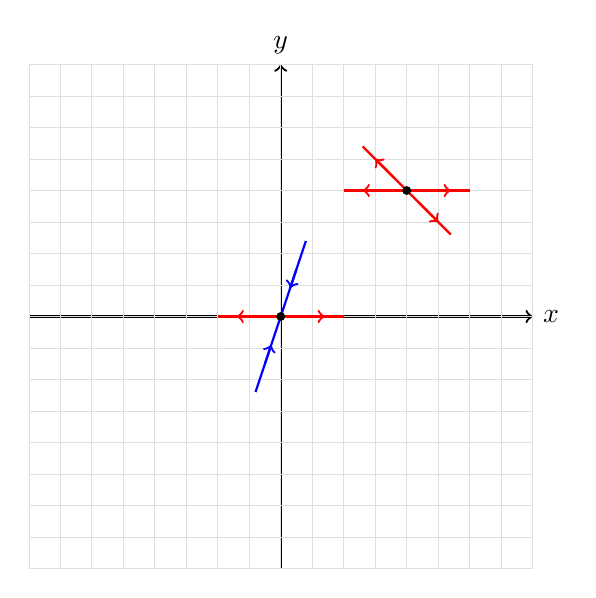
\begin{tikzpicture}[scale=0.8]
    % Axes
    \draw[->,thick] (-4,0)--(4,0) node[right]{$x$};
    \draw[->,thick] (0,-4)--(0,4) node[above]{$y$};
    
    % Grid
    \draw[step=0.5cm,very thin,gray!25] (-4,-4) grid (4,4);
    
    
    % Saddle at (0,0)
    \draw[red, thick] (-1,0)--(1,0);
    \draw[blue, thick] (-0.4,-1.2)--(0.4,1.2);
    \draw[->, red, thick] (0.5,0)--(0.7,0);
    \draw[->, red, thick] (-0.5,0)--(-0.7,0);
    \draw[->, blue, thick] (0.25,0.75)--(0.15,0.45);
    \draw[->, blue, thick] (-0.25,-0.75)--(-0.15,-0.45);

    
    % Unstable node at (2,2)
    \draw[red, thick] (1,2)--(3,2);
    \draw[red, thick] (2.7,1.3)--(1.3,2.7);
    \draw[->, red, thick] (2.5,2)--(2.7,2);
    \draw[->, red, thick] (1.5,2)--(1.3,2);
    \draw[->, red, thick] (2.2,1.8)--(2.5,1.5);
    \draw[->, red, thick] (1.8,2.2)--(1.5,2.5);

    % Equilibria
    \fill (0,0) circle (2pt);
    \fill (2,2) circle (2pt);
\end{tikzpicture}
\end{center}
%-------------------------------------------------------------
Then extend all solution curves. The solution curves from each equilibrium may connect to form one solution curve. Keep in mind that two solution curves can never intersect. Try to fill the phase plane with solution curves.

\begin{center}
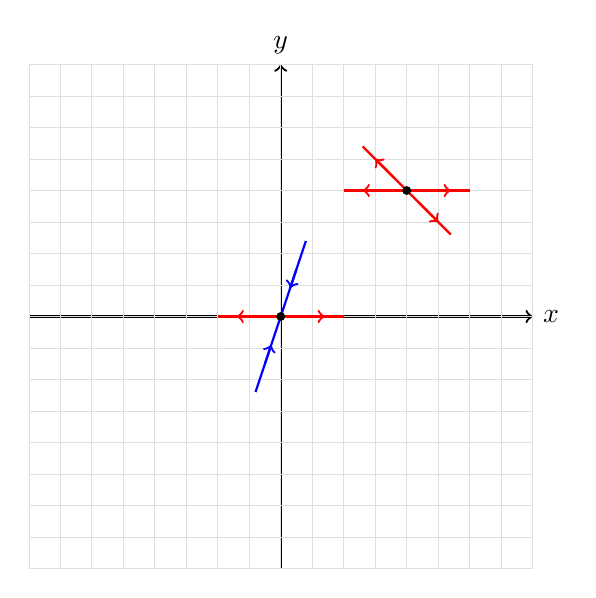
\begin{tikzpicture}[scale=0.8]
    % Axes
    \draw[->,thick] (-4,0)--(4,0) node[right]{$x$};
    \draw[->,thick] (0,-4)--(0,4) node[above]{$y$};
    
    % Grid
    \draw[step=0.5cm,very thin,gray!25] (-4,-4) grid (4,4);
    
    
    % Saddle at (0,0)
    \draw[red, thick] (-1,0)--(1,0);
    \draw[blue, thick] (-0.4,-1.2)--(0.4,1.2);
    \draw[->, red, thick] (0.5,0)--(0.7,0);
    \draw[->, red, thick] (-0.5,0)--(-0.7,0);
    \draw[->, blue, thick] (0.25,0.75)--(0.15,0.45);
    \draw[->, blue, thick] (-0.25,-0.75)--(-0.15,-0.45);

    
    % Unstable node at (2,2)
    \draw[red, thick] (1,2)--(3,2);
    \draw[red, thick] (2.7,1.3)--(1.3,2.7);
    \draw[->, red, thick] (2.5,2)--(2.7,2);
    \draw[->, red, thick] (1.5,2)--(1.3,2);
    \draw[->, red, thick] (2.2,1.8)--(2.5,1.5);
    \draw[->, red, thick] (1.8,2.2)--(1.5,2.5);

    % Equilibria
    \fill (0,0) circle (2pt);
    \fill (2,2) circle (2pt);
\end{tikzpicture}
\end{center}
\noindent\textbf{Comment about ambiguity:} The linearization tells us exactly what happens near an equilibrium, but it tells us very little about what happens far away. When sketching nonlinear phase portraits, we are not drawing exact solutions—we are constructing a consistent picture using local linear behavior and global rules, such as non-intersection of trajectories.

%-------------------------------------------------------------
\end{document}